\documentclass{article}
\usepackage{fontspec}
\setsansfont{Helvetica}
\renewcommand{\familydefault}{\sfdefault}
\usepackage{tikz}
\usetikzlibrary{arrows.meta}
\pagestyle{empty}
\definecolor{cA}{HTML}{1F77B4}
\definecolor{cB}{HTML}{FF7F0E}
\definecolor{lookup}{HTML}{2A78D6}
\definecolor{lookuplight}{HTML}{9DC1EC}
\definecolor{write}{HTML}{EB6834}
\definecolor{writelight}{HTML}{F5B597}
\definecolor{ink}{HTML}{0B0B0B}
\definecolor{inktwo}{HTML}{52514E}
\definecolor{gridc}{HTML}{E4E3DF}
\definecolor{axisc}{HTML}{8F8E89}
\definecolor{refc}{HTML}{3D3C39}
\tikzset{
  tick/.style={font=\footnotesize, text=black, inner sep=1.5pt},
  lab/.style={font=\small, text=ink, inner sep=1.5pt},
  note/.style={font=\footnotesize, text=inktwo, inner sep=1.5pt},
  ser/.style={line width=1.4pt, line cap=round, line join=round},
  thin/.style={line width=0.9pt, line cap=round, line join=round},
  ref/.style={line width=0.8pt, draw=refc, dash pattern=on 3pt off 2pt},
}
\begin{document}
\setbox0=\hbox{%
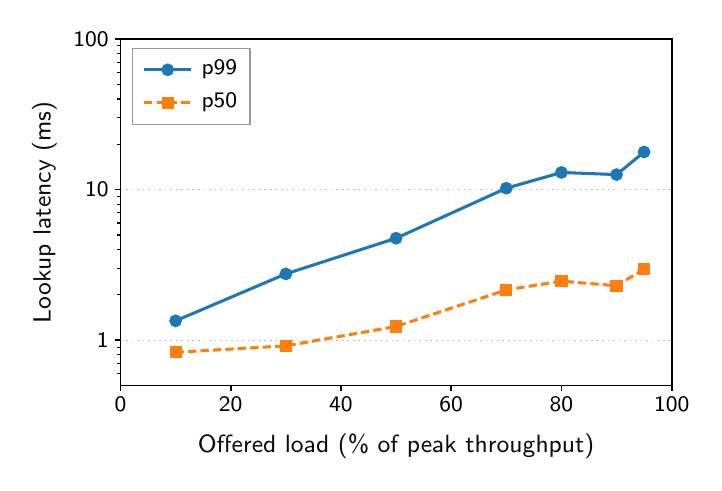
\begin{tikzpicture}[x=1cm,y=1cm]
\draw[black!25, line width=0.4pt, dash pattern=on 0.6pt off 1.4pt] (0.000,0.576) -- (7.000,0.576);
\draw[black, line width=0.6pt] (0.000,0.576) -- (-0.070,0.576);
\node[tick, anchor=east] at (-0.090,0.576) {1};
\draw[black!25, line width=0.4pt, dash pattern=on 0.6pt off 1.4pt] (0.000,2.488) -- (7.000,2.488);
\draw[black, line width=0.6pt] (0.000,2.488) -- (-0.070,2.488);
\node[tick, anchor=east] at (-0.090,2.488) {10};
\draw[black!25, line width=0.4pt, dash pattern=on 0.6pt off 1.4pt] (0.000,4.400) -- (7.000,4.400);
\draw[black, line width=0.6pt] (0.000,4.400) -- (-0.070,4.400);
\node[tick, anchor=east] at (-0.090,4.400) {100};
\draw[black, line width=0.4pt] (0.000,0.151) -- (-0.040,0.151);
\draw[black, line width=0.4pt] (0.000,0.279) -- (-0.040,0.279);
\draw[black, line width=0.4pt] (0.000,0.390) -- (-0.040,0.390);
\draw[black, line width=0.4pt] (0.000,0.488) -- (-0.040,0.488);
\draw[black, line width=0.4pt] (0.000,1.151) -- (-0.040,1.151);
\draw[black, line width=0.4pt] (0.000,1.488) -- (-0.040,1.488);
\draw[black, line width=0.4pt] (0.000,1.727) -- (-0.040,1.727);
\draw[black, line width=0.4pt] (0.000,1.912) -- (-0.040,1.912);
\draw[black, line width=0.4pt] (0.000,2.064) -- (-0.040,2.064);
\draw[black, line width=0.4pt] (0.000,2.192) -- (-0.040,2.192);
\draw[black, line width=0.4pt] (0.000,2.303) -- (-0.040,2.303);
\draw[black, line width=0.4pt] (0.000,2.400) -- (-0.040,2.400);
\draw[black, line width=0.4pt] (0.000,3.063) -- (-0.040,3.063);
\draw[black, line width=0.4pt] (0.000,3.400) -- (-0.040,3.400);
\draw[black, line width=0.4pt] (0.000,3.639) -- (-0.040,3.639);
\draw[black, line width=0.4pt] (0.000,3.824) -- (-0.040,3.824);
\draw[black, line width=0.4pt] (0.000,3.976) -- (-0.040,3.976);
\draw[black, line width=0.4pt] (0.000,4.104) -- (-0.040,4.104);
\draw[black, line width=0.4pt] (0.000,4.215) -- (-0.040,4.215);
\draw[black, line width=0.4pt] (0.000,4.313) -- (-0.040,4.313);
\draw[black, line width=0.6pt] (0.000,0.000) -- (0.000,-0.070);
\node[tick, anchor=north] at (0.000,-0.090) {0};
\draw[black, line width=0.6pt] (1.400,0.000) -- (1.400,-0.070);
\node[tick, anchor=north] at (1.400,-0.090) {20};
\draw[black, line width=0.6pt] (2.800,0.000) -- (2.800,-0.070);
\node[tick, anchor=north] at (2.800,-0.090) {40};
\draw[black, line width=0.6pt] (4.200,0.000) -- (4.200,-0.070);
\node[tick, anchor=north] at (4.200,-0.090) {60};
\draw[black, line width=0.6pt] (5.600,0.000) -- (5.600,-0.070);
\node[tick, anchor=north] at (5.600,-0.090) {80};
\draw[black, line width=0.6pt] (7.000,0.000) -- (7.000,-0.070);
\node[tick, anchor=north] at (7.000,-0.090) {100};
\draw[line width=1.1pt, line join=round, draw=cB, dash pattern=on 3pt off 1.5pt] (0.700,0.422) -- (2.100,0.504) -- (3.500,0.750) -- (4.900,1.215) -- (5.600,1.326) -- (6.300,1.267) -- (6.650,1.479);
\draw[line width=1.1pt, line join=round, draw=cA] (0.700,0.822) -- (2.100,1.418) -- (3.500,1.871) -- (4.900,2.506) -- (5.600,2.706) -- (6.300,2.679) -- (6.650,2.966);
\filldraw[fill=cB, draw=cB, line width=0.8pt] (0.700,0.422) +(-1.8pt,-1.8pt) rectangle +(1.8pt,1.8pt);
\filldraw[fill=cB, draw=cB, line width=0.8pt] (2.100,0.504) +(-1.8pt,-1.8pt) rectangle +(1.8pt,1.8pt);
\filldraw[fill=cB, draw=cB, line width=0.8pt] (3.500,0.750) +(-1.8pt,-1.8pt) rectangle +(1.8pt,1.8pt);
\filldraw[fill=cB, draw=cB, line width=0.8pt] (4.900,1.215) +(-1.8pt,-1.8pt) rectangle +(1.8pt,1.8pt);
\filldraw[fill=cB, draw=cB, line width=0.8pt] (5.600,1.326) +(-1.8pt,-1.8pt) rectangle +(1.8pt,1.8pt);
\filldraw[fill=cB, draw=cB, line width=0.8pt] (6.300,1.267) +(-1.8pt,-1.8pt) rectangle +(1.8pt,1.8pt);
\filldraw[fill=cB, draw=cB, line width=0.8pt] (6.650,1.479) +(-1.8pt,-1.8pt) rectangle +(1.8pt,1.8pt);
\filldraw[fill=cA, draw=cA, line width=0.8pt] (0.700,0.822) circle (1.9pt);
\filldraw[fill=cA, draw=cA, line width=0.8pt] (2.100,1.418) circle (1.9pt);
\filldraw[fill=cA, draw=cA, line width=0.8pt] (3.500,1.871) circle (1.9pt);
\filldraw[fill=cA, draw=cA, line width=0.8pt] (4.900,2.506) circle (1.9pt);
\filldraw[fill=cA, draw=cA, line width=0.8pt] (5.600,2.706) circle (1.9pt);
\filldraw[fill=cA, draw=cA, line width=0.8pt] (6.300,2.679) circle (1.9pt);
\filldraw[fill=cA, draw=cA, line width=0.8pt] (6.650,2.966) circle (1.9pt);
\draw[black, line width=0.6pt] (0.000,0.000) rectangle (7.000,4.400);
\node[lab, anchor=north] at (3.500,-0.550) {Offered load (\% of peak throughput)};
\node[lab, rotate=90, anchor=south] at (-0.750,2.200) {Lookup latency (ms)};
\draw[fill=white, draw=black!40, line width=0.4pt] (0.150,4.280) rectangle (1.645,3.320);
\draw[line width=1.1pt, line join=round, draw=cA] (0.300,4.010) -- (0.900,4.010);
\filldraw[fill=cA, draw=cA, line width=0.8pt] (0.600,4.010) circle (1.9pt);
\node[tick, anchor=west] at (0.970,4.010) {p99};
\draw[line width=1.1pt, line join=round, draw=cB, dash pattern=on 3pt off 1.5pt] (0.300,3.590) -- (0.900,3.590);
\filldraw[fill=cB, draw=cB, line width=0.8pt] (0.600,3.590) +(-1.8pt,-1.8pt) rectangle +(1.8pt,1.8pt);
\node[tick, anchor=west] at (0.970,3.590) {p50};
\end{tikzpicture}}%
\pdfvariable horigin=0pt
\pdfvariable vorigin=0pt
\pagewidth=\dimexpr\wd0+8pt\relax
\pageheight=\dimexpr\ht0+\dp0+8pt\relax
\shipout\vbox{\kern4pt\hbox{\kern4pt\box0\kern4pt}\kern4pt}
\end{document}
